\chapter{Architecture}
\label{ch:architecture}
Slips is a modular software. Each module is designed to perform a specific detection in the network traffic.\cite{slips}
However, the modules can be also used to directly extend Slips with any additional functionality. 
Fides was designed for seamless interoperability with Slips and in addition to generic trust model, we developed the Fides module for Slips.
In this chapter, we describe architecture of Fides, how does it interact with the network as well as with Slips.

\begin{figure}[ht]
    \centering
    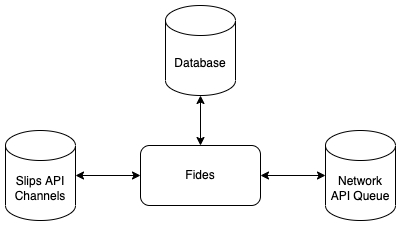
\includegraphics[width=0.7\textwidth]{assets/high_architecture.png}
    \caption{High Level Architecture}
    \label{fig:high-level-architecture}
\end{figure}

From the high level perspective (figure \ref{fig:high-level-architecture}), trust model communicates with two different entities - Slips and network layer.
For both parts, Fides exposes and consumes an API\footnote{Application Programming Interface - a software interface that is used for communication between two programs} that is built using Redis\footnote{In-memory data structure store, supports asynchronous channels and publish-subscribe model.} channels.
We choose to employ Redis channels, as the medium that allows communication between the network layer and Fides and allows them to use their respective APIs.
Because Slips already uses Redis for its internal communication between module, it brings no additional overhead to run Fides with its network layer.

Moreover, Fides stores trust related data (past interactions, cached network opinions, service trust, recommendations etc.) inside the database.
The database layer was implemented as an abstract part and can be easily replaced in the future.
As of now, we have two different implementations - in memory database and database that stores data in Redis, if the persistence is needed.

\section{Fides \& Network Access}
\label{sec:fides-and-network-access}

\begin{figure}[ht]
    \centering
    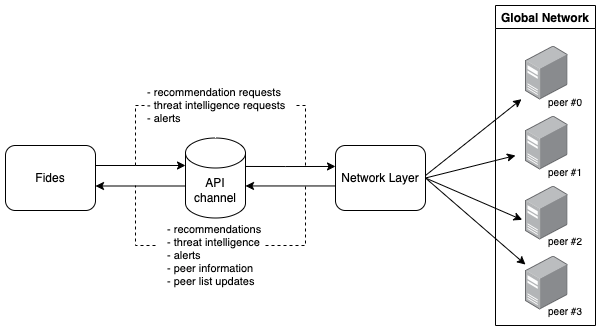
\includegraphics[width=1.0\textwidth]{assets/tl_api_nl.png}
    \caption{Communication between Fides and Network Layer}
    \label{fig:fides-api-network}
\end{figure}

Fides itself is a trust model, set of equations and data storage for interaction history. 
It does not interact with the network directly, bur rather it exposes an API which can be used either to receive the information from the network or for sending the requests back to the network.
Thanks to this design, where all business logic is separated from the network layer, Fides is highly modular and it does not depend on the network layer implementation.
Network layer then performs all data transfers and remote peers communications.
It also facilitates finding new peers and ensuring that all requests from Fides are dispatched to correct recipients.
In the eyes of Fides, network layer is a \textit{blackbox} and it does not need to know, how is the network layer implemented.
See figure \ref{fig:fides-api-network} for high level overview of the communication.

How does the network layer work in detail and what protocols are used describes Martin Řepa in his master's thesis \cite{nl}.
